\subsection{Operating conditions}\label{subsec:operating-conditions}

\subsubsection{Client}
The client consists of the \textit{browser-client}, the browser extension that is used to create replics, and the \textit{web-client}, the web app that is used for account management and content viewing.
Both must be usable under the following environments:

\begin{enumerate}
    \item Chromium-based browsers
    \item Firefox
\end{enumerate}

\subsubsection{Server and Database}
The server is meant for unlimited runtime.
The following requirements are imposed:
\begin{itemize}
    \item Debian 12.
    \item Access to the internet with speeds of at least 50mb/s up- and download.
    \item Latency below 50ms.
    \item Minimum storage of 5GB\@.
    \item Minimum memory of 4GB\@.
\end{itemize}

The server must be exposed to the internet via a fixed domain, that is given to the server via configuration.
Other systems may be supported.

\subsection{State overview}\label{subsec:state-management}
\subsubsection{User}
As specified in~\ref{ac:accounts:5},\ref{ac:accounts:4}, users and their account have a specific state.
This is visualized in Figure~\ref{fig:user-state}.

\begin{figure}
    \centering
    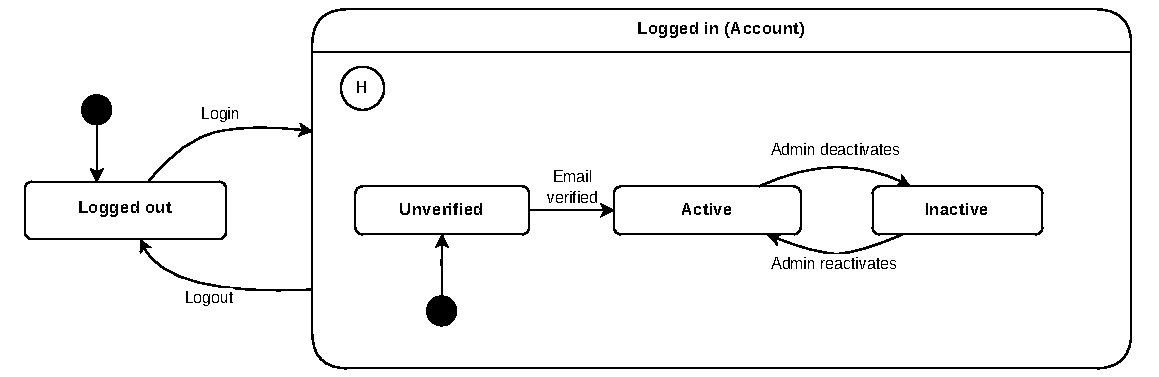
\includegraphics[width=\linewidth]{user-state}
    \caption{State of a user and its' account.}
    \label{fig:user-state}
\end{figure}

\subsubsection{Replic}
As specified in~\ref{ac:replics:5}, a replic can be in multiple states.
This is visualized in Figure~\ref{fig:replic-state}.

\begin{figure}
    \centering
    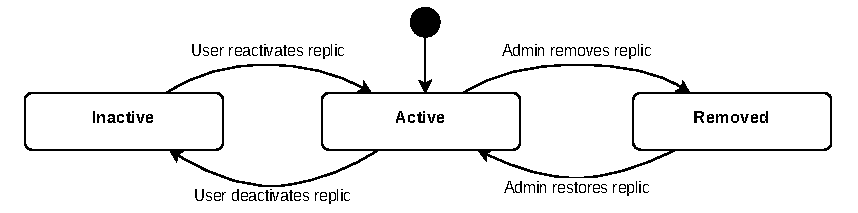
\includegraphics[width=\linewidth]{replic-state}
    \caption{State of a replic.}
    \label{fig:replic-state}
\end{figure}

\subsection{Use-cases}\label{subsec:use-cases}

\subsubsection{Account management}
\begin{figure}
    \centering
    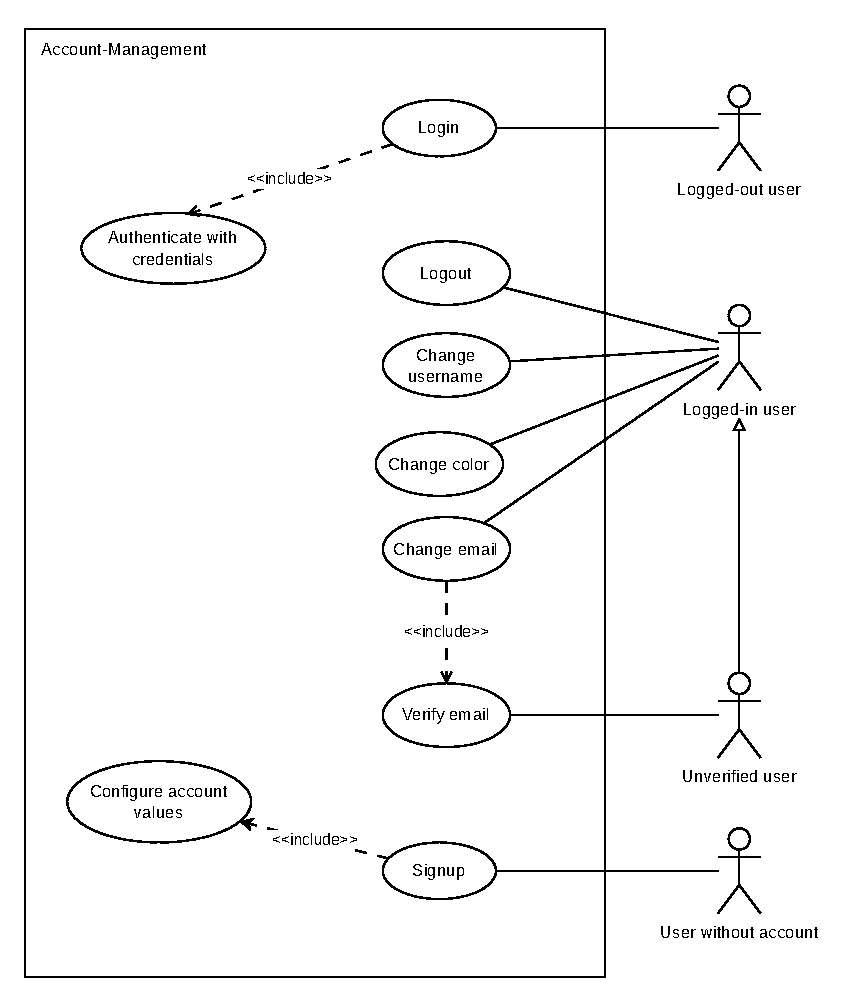
\includegraphics{uc-account-management}
    \caption{Use-cases for the account-management.}
    \label{fig:account-management}
\end{figure}

Figure~\ref{fig:account-management} shows the usecases related to authentication and management of the account.
We differentiate between
\begin{itemize}
    \item \textit{Logged-out users}: Users who are currently not logged in, but have access to crdentials to an account.
    \item \textit{Deactivated user}: Users who deactivated their own account.
    \item \textit{Logged-in user}: Users who are currently logged in and can perform actions.
    \item \textit{User without account}: Users who have never interacted with the system and can create a new account.
    \item \textit{Unverified user}: Users who are logged into an account that doesn't have their email verified.
\end{itemize}

\subsubsection{Admin panel}
\begin{figure}
    \centering
    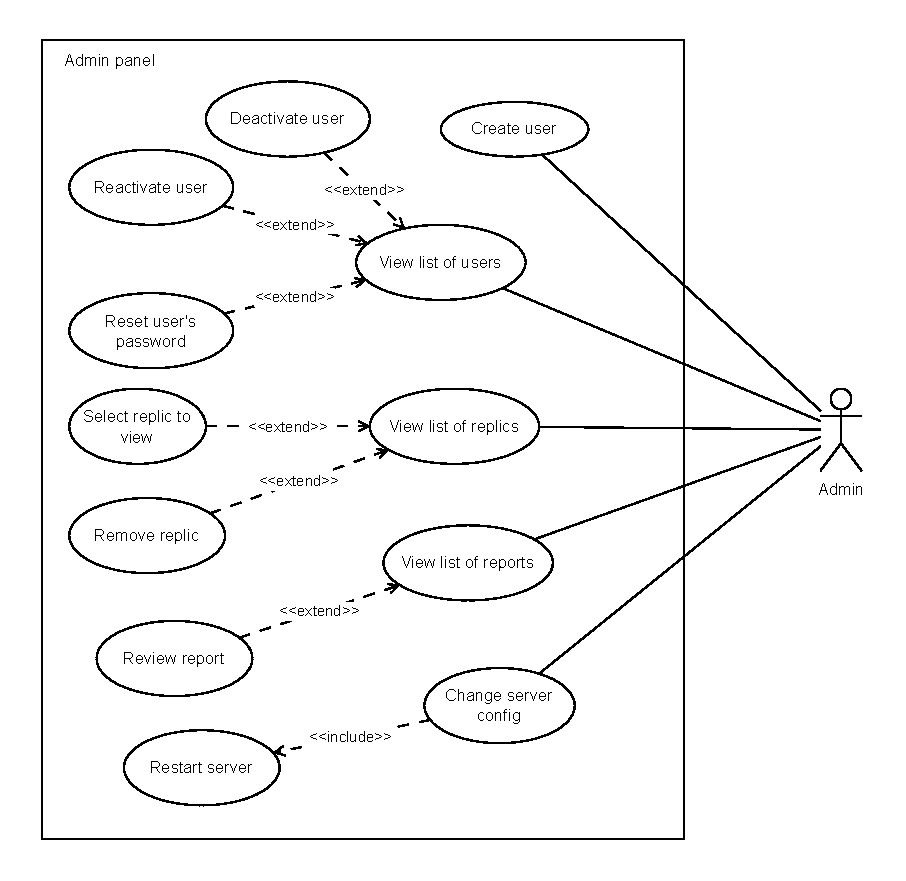
\includegraphics{uc-admin-panel}
    \caption{Use-cases for the admin-panel.}
    \label{fig:admin-panel}
\end{figure}

Figure~\ref{fig:admin-panel} shows the usecases related to the admin panel.
The only users that can interact with this subsystem are admin users.
Admin users have access to a list of users, replics and reports.
For each the have access to specific context actions to manipulate single items.

\subsubsection{Replic creation}
\begin{figure}
    \centering
    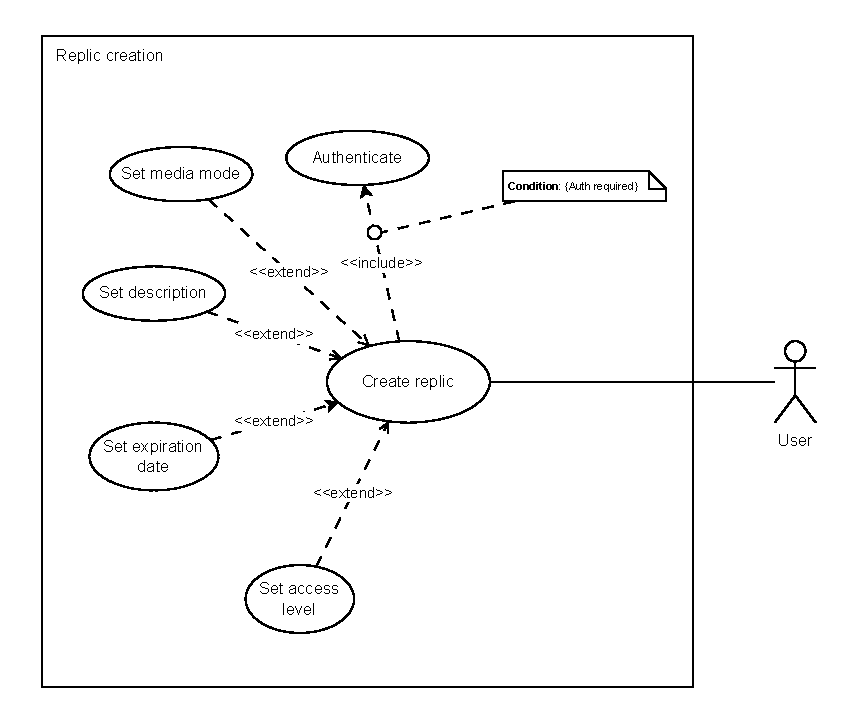
\includegraphics{uc-replic-creation}
    \caption{Use-cases for the replic-creation.}
    \label{fig:replic-creation}
\end{figure}

Figure~\ref{fig:replic-creation} shows the usecases for the subsystem that manages creating a single replic.
The base usecase of \("\)Create replic\("\) has many includes, that correspond to configurations of the replic that will be created.
\("\)Authenticate\("\) is only necessary if creating a replica requires authentication, a server-wide setting.

\subsubsection{Replic management}
\begin{figure}
    \centering
    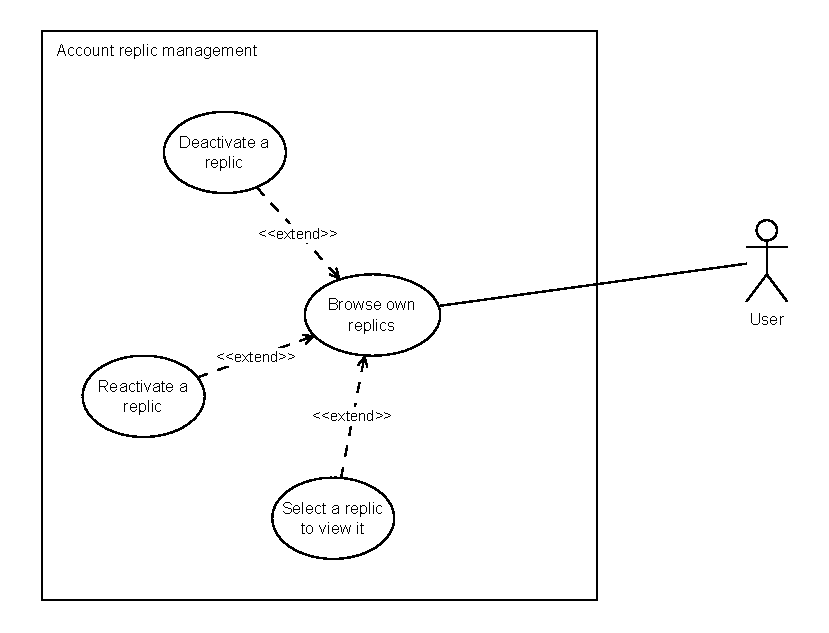
\includegraphics{uc-replic-management}
    \caption{Use-cases for the replic-management.}
    \label{fig:replic-management}
\end{figure}

Figure~\ref{fig:replic-management} shows the usecases for managing the replics of an account.
The main usecase \("\)Browse own replics\("\) has three context actions that allow to deactivate a replic, to reactivate a deactivated replic and to select and view a replic.

\subsubsection{Replic viewing}
\begin{figure}
    \centering
    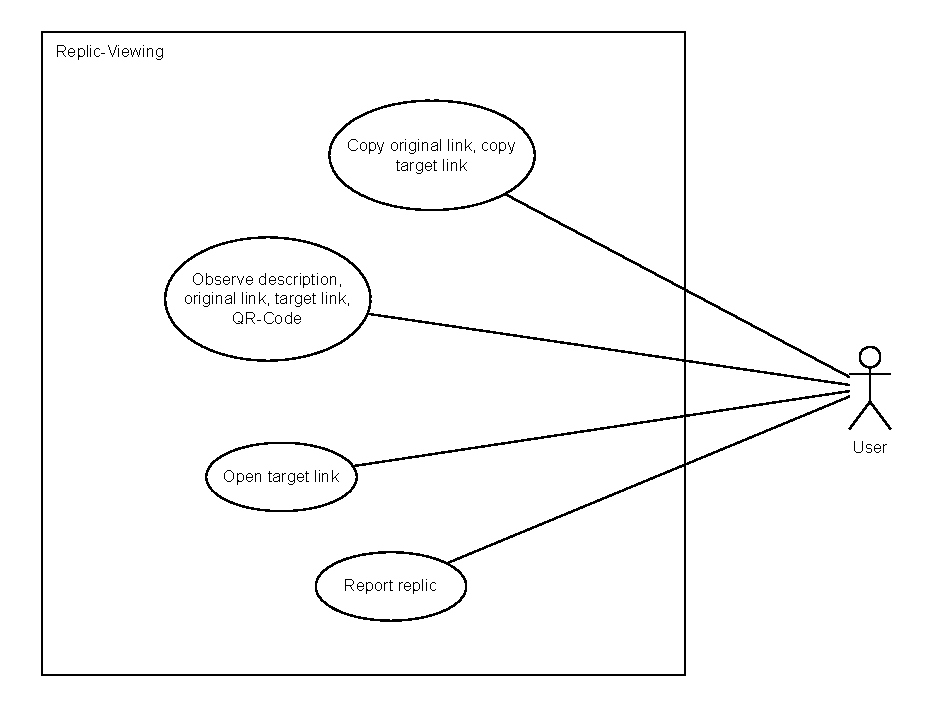
\includegraphics{uc-replic-viewing}
    \caption{Use-cases for the replic-viewing.}
    \label{fig:replic-viewing}
\end{figure}

Figure~\ref{fig:replic-viewing} shows the usecases for when a replic is being viewn.
The context actions are related to accessing the archived media, sharing and repeorting it.

\subsubsection{Miscellaneous}
\begin{figure}
    \centering
    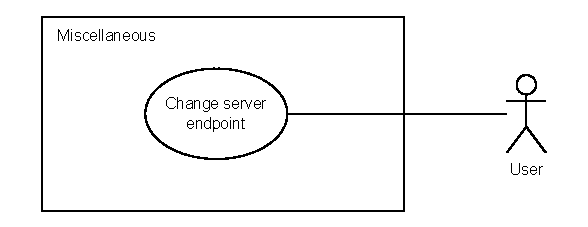
\includegraphics{uc-miscellaneous}
    \caption{Miscellaneous use-cases.}
    \label{fig:miscellaneous}
\end{figure}

Figure~\ref{fig:miscellaneous} shows general usecases that are not part of a specific subsystem.